
\section{Batch RL Setting}
We test the performance of our algorithm in a Batch RL setting.
To this end, we make use the D4RL dataset \cite{d4rl}, a recent suite of tasks and datasets for
benchmarking progress in offline RL.
\subsection{Half-Cheetah}
We first use the Gym-Mujoco benchmark tasks, specifically \textit{HalfCheetah}.
In the \textit{HalfCheetah} environment, a 2D chetah needs to learn to run.
The observation space has 17 dimensions (accounting for velocity and position of the joints)
The control space has a dimensionality of 6, constrained between -1 and 1, 
controlling the torques applied to the joints.

\subsubsection{Dataset}
We use the \textit{halfcheetah-medium-v0} dataset, which consists of data generated by
training a policy online using a standard RL algorithm (SAC) for a few steps till it reaches 
approximately 1/3 the performance of the expert. Then, they stop the training
and collecting 1M samples from this partially trained policy.

The environment is deterministic, so to proof the performance of our algorithm, we modify the environment to
add a source of uncertainty.
We introduce stochasticity in the original cost function in a way that 
makes the environment stochastic enough to have a meaningful assessment of risk in terms of 
tail performance.
A reward of $R_v=-100$ is given with probability 0.05, if the velocity of the cheetah is greater than 4.
Due to the fact that there is no direct access to the velocity of the cheetah from the observations,
we reran the environment interactions from the dataset in open-loop, to collect the desired information and 
modify the rewards accordingly.
The modified dataset was used to train the algorithm in an off-line way.

In the following we show the evaluation during training for both \textit{Mean} and
\textit{CVaR}.
Specifically, every 1000 training steps, we evaluate the current policy for 5 episodes.
Only for this evaluation process, we allow the agent to interact with the environment.
The environment is modified with a RewardWrapper to introduce the stochasticity on the reward for
high velocities.
During evaluation, to ensure the deterministic nature of the policy, 
the latent vector is not sampled from a gaussian, but a vector of zeros is used instead.

During this 5 evaluation episodes, we compute the mean of the cumulative rewards,
the CVaR with a confidence level of 0.1 and also the mean of the number of times the 
maximum velocity is exceeded. 

After training, we used the final policies and deployed them in the noisy environment for 20 episodes 
200 timesteps each. An histogram of the resulting cumulative rewards is added below showing
how the \textit{Mean} algorithm obtain in average higher rewards, but in some scenarios it 
obtains really low results, whereas the \textit{CVaR} performs in average worse than \textit{Mean} 
but the conditional value at risk is higher than for the \textit{Mean}.
Results are shown below.



\begin{figure}[ht]
        \centering
        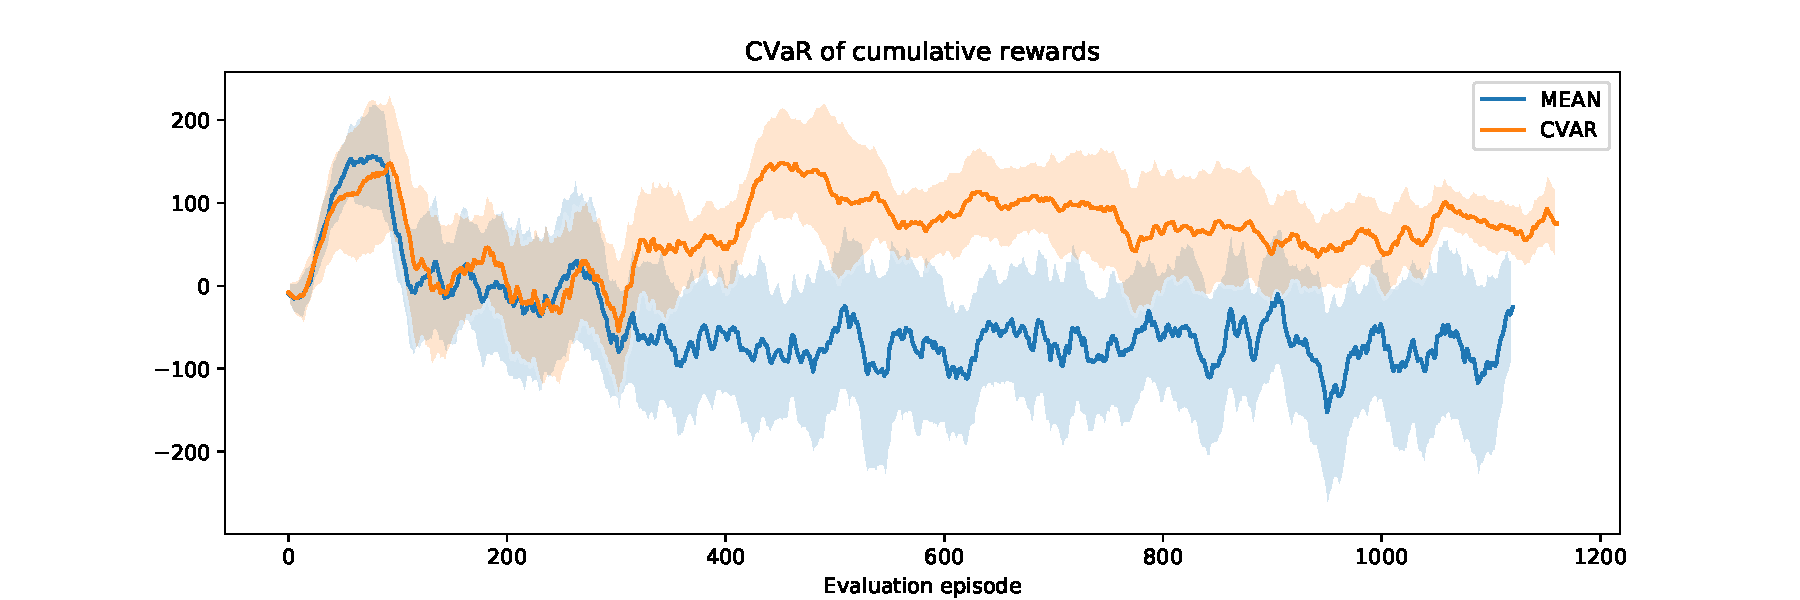
\includegraphics[width=0.8\textwidth]{images/Cheetah_offpolicy_medium/cvar_train_withstds.pdf}
        \caption{CVaR$_\alpha=0.1$ of the cumulative rewards over 5 evaluation episodes.
        Every point corresponds to one evaluation process performed every 1000 steps of training}
        \label{cvar_cheetah}
    
\end{figure}

\begin{figure}[ht]
    \centering
    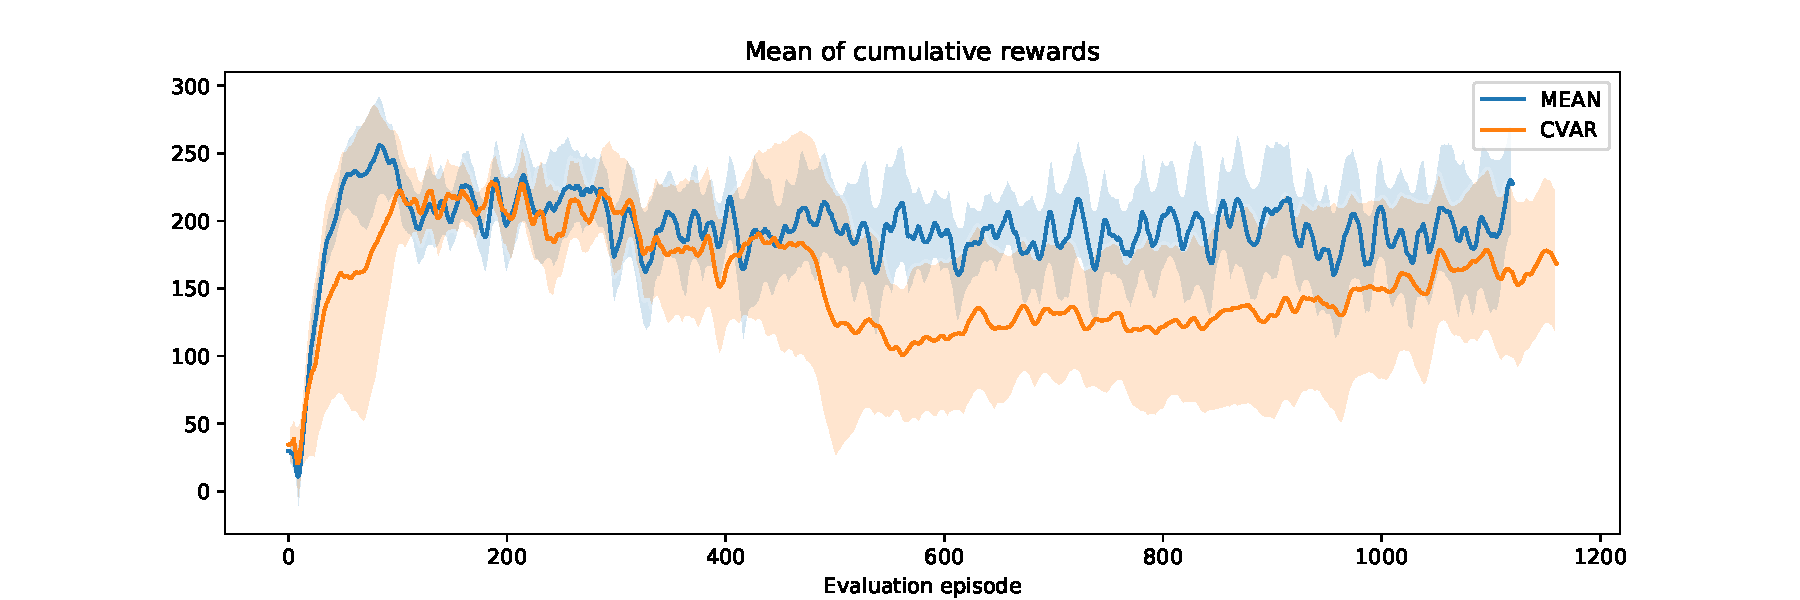
\includegraphics[width=0.8\textwidth]{images/Cheetah_offpolicy_medium/mean_train_withstds.pdf}
    \caption{Mean of the cumulative rewards over 5 evaluation episodes. Every point corresponds
    to one evaluation process performed every 1000 steps of training}
    \label{mean_cheetah}

\end{figure}



\begin{figure}[ht]
    \centering
    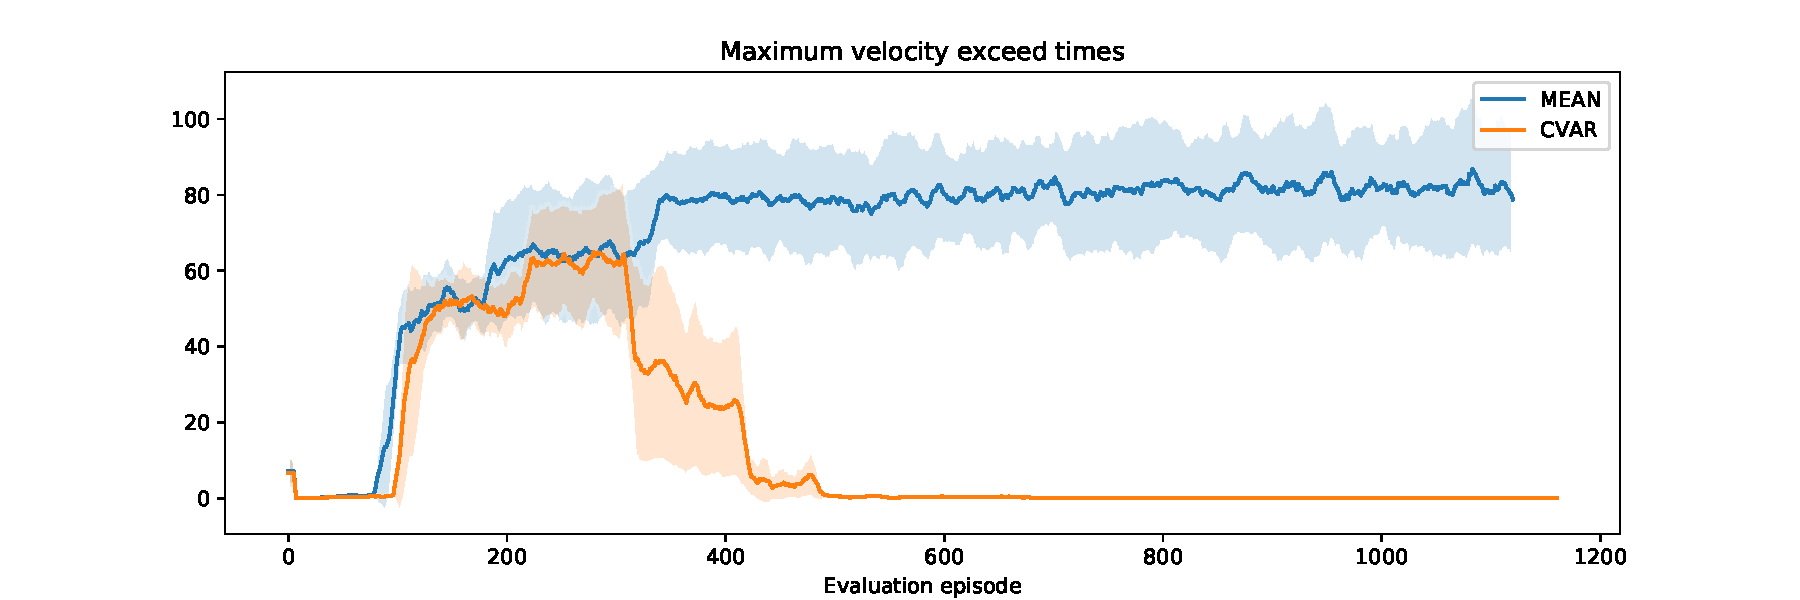
\includegraphics[width=0.8\textwidth]{images/Cheetah_offpolicy_medium/times_exceedvel_withstds.pdf}
    \caption{Mean of number of times the maximum velocity was exceeded over 5 evaluation episodes.
    Every point corresponds to one evaluation process performed every 1000 steps of training}
    \label{vel_exceed_cheetah}

\end{figure}

\begin{figure}[ht]
    \centering
    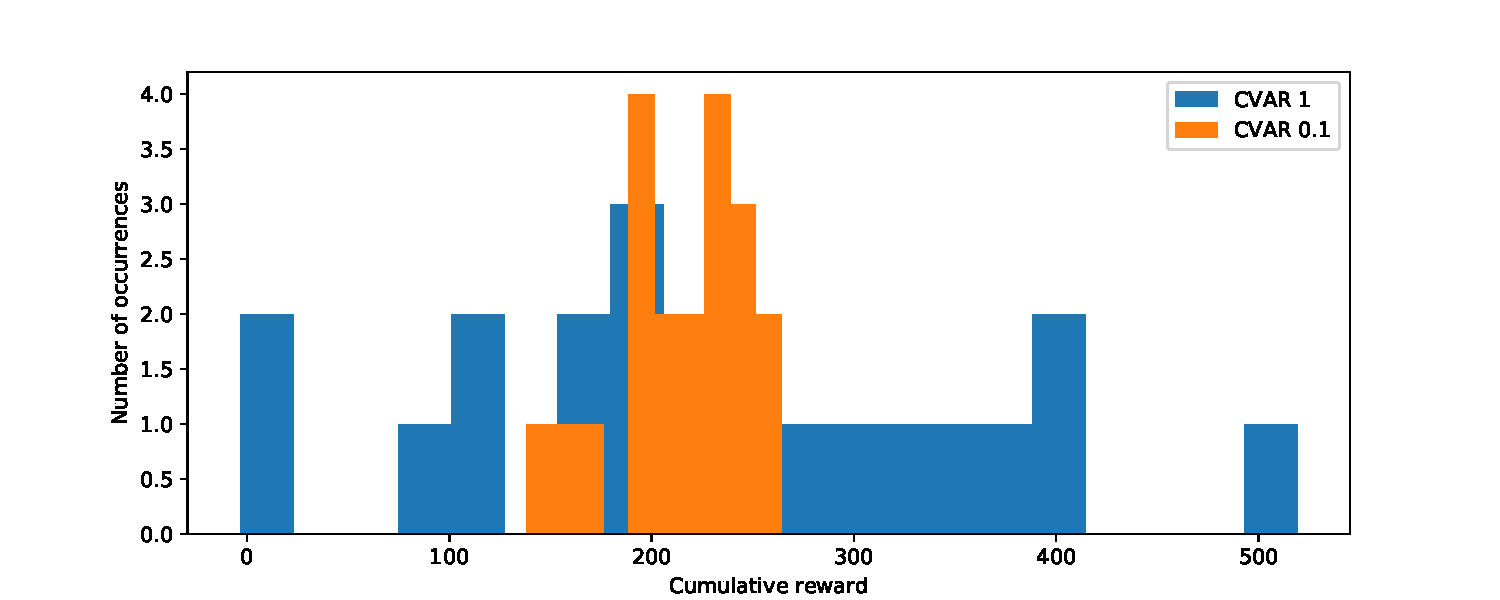
\includegraphics[width=0.8\textwidth]{images/Cheetah_offpolicy_medium/hist_evaluation_numevalsteps200.pdf}
    \caption{Histogram of cumulative rewards during 200 time steps using the trained final policies}
    \label{hist_cum_rewards200steps_cheetah}

\end{figure}

\clearpage

\subsection{Walker}
Add more environments. To be decided
\subsection{Medical environment}
Add more environments. To be decided